%%%%%%%%%%%%%%%%%%%
% Import Setting  %
%%%%%%%%%%%%%%%%%%%

\documentclass[
    paper=a4,
    fontsize=12pt,
    parskip=half,
    headheight=32pt,
    DIV=12,
    BCOR=3mm
  ]{scrartcl}

  \usepackage[english, ngerman]{babel}
  \usepackage[utf8]{inputenc}
  \usepackage{amsmath}
  \usepackage{graphicx}
  \usepackage{bookmark}
  \usepackage{array}
  %usepackage{showframe} % to see the frame of the pdf
  \usepackage[a4,center,cam]{crop} % set size of page frame. Synergy with Koma-Script

  % Allows adding inline-code
  \usepackage{listings}

  % Allow direct copy&paste from the pdf
  \usepackage[T1]{fontenc}
  \usepackage[utf8]{inputenc}

  \PassOptionsToPackage{colorlinks=true,linkcolor=blue}{hyperref}
  %\usepackage[colorlinks=true,linkcolor=blue]{hyperref}

  % Header and Footer
  \usepackage[headsepline=0.4pt,plainfootsepline]{scrlayer-scrpage}
  \pagestyle{scrheadings}
  \clearpairofpagestyles

  \ihead{Reverse Engineering}
  \ohead{
\includegraphics[width=2cm]{../img/HM_Logo.jpg}}
  \usepackage{lastpage}
  \cfoot{Seite \pagemark\hspace{0.9pt} von \hspace{0.9pt}\pageref{LastPage}}

\begin{document}

%%%%%%%%%%%%%%%
% Titelseite  %
%%%%%%%%%%%%%%%
\begin{titlepage}
    \newcommand{\HRule}{\rule{\linewidth}{0.35mm}} % Defines a new command for the horizontal lines

    \center% Center everything on the page

    \textsc{\LARGE Reverse Engineering}\\[0.7cm]

    \begin{figure} [!ht]
        \centering
        
\includegraphics[width=5cm]{../img/HM_Logo.jpg}
    \end{figure}

    \textsc{\Large Übung 1 - Gruppe 3}\\[0.7cm]

    \HRule

    \begin{tabular}{*{3}{>{\centering}p{.25\textwidth}}}
        Ludwig Karpfinger & Armin Jeleskovic & Valentin Altemeyer \tabularnewline
        \url{ludwig.karpfinger@hm.edu} & \url{a.jeleskovic@hm.edu} & \url{valentin.altemeyer@hm.edu}
    \end{tabular}\par
    \HRule

    \textsc{}\\[0.3cm]

    \let\endtitlepage\relax

\end{titlepage}

%%%%%%%%%%%%%%%%%%%%%%%%%%%%%%
% Aufgaben ab hier einfügen  %
%%%%%%%%%%%%%%%%%%%%%%%%%%%%%%
\section*{Aufgabe 1 Zip Datei entpacken}

\subsection*{a) Zip Datei entpacken}

\subsubsection*{UI Tool:}

Das vorinstallierte UI Tool in Nautilus ist der Meinung, dass die vorliegende Datei passwortgeschützt ist.
Das Öffnen ist nicht möglich.

\subsubsection*{CLI Tool:}

\begin{lstlisting}[language=bash]
    $ unzip packed.zip
\end{lstlisting}

Die Fehlermeldung lautet \textit{invalid compressed data to inflate}.
Man könnte vermuten, dass dies an einer ungültigen Bytesquenz in der Dateistruktur liegt.
Die Datei scheint nicht völlig unbrauchbar zu sein, da folgender Befehl ergibt, dass die zip File
eine Textdatei namens Unpackme.txt enthält:

\begin{lstlisting}[language=bash]
    $ unzip -l packed.zip
\end{lstlisting}

\subsection*{b) ZIP reparieren}

Eine ZIP-File folgt der Dateistruktur von PKZip\footnote{\url{https://users.cs.jmu.edu/buchhofp/forensics/formats/pkzip.html}}.

%Eine ZIP file hat folgenden Aufbau:
%\begin{enumerate}
%    \item Local File Header
%    \begin{enumerate}
%        \item Signature \textit{504b 0304}
%    \end{enumerate}
%    \item File Data
%    \item Data descriptor (optional)
%    \item Archive decryption header (optional)
%    \item Archive extra data record (optional)
%    \item Central directory
%    \item \begin{enumerate}
%        \item Signature \textit{504b 0102}
%    \end{enumerate}
%    \item End of central directory
%    \begin{enumerate}
%        \item Signature \textit{504b 0506}
%    \end{enumerate}
%\end{enumerate}

Das \textit{Extra Field} in einer Zip Datei ist vorhanden, um zusätzliche Informationen zu speichern.
Es wird der Tipp gegeben, dass die Längenangabe im \textit{extra field} auf 28 bytes gesetzt werden muss.
Das Tool \textit{hexedit} kann die Bytes anpassen.

Nun kann die Zip file entpackt werden.
Obwohl das möglich ist, wird die Fehlermeldung
\textit{invalid zip file with overlapped components (possible zip bomb)} ausgegeben.

Dies konnte nicht gelöst werden.

\subsection*{c) Inhalt ausgeben}

Der Inhalt lautet: \textit{Wenn man es weiß ist es eigentlich ganz einfach.}

%%%%%%%%%%%%%%
% Aufgabe 2  %
%%%%%%%%%%%%%%
\section*{Aufgabe 2 Einstieg in ELF Reversing}

\subsection*{a) main Methode in stripped File}

Der Entry Point der Datei findet man durch den gdb Debugger heraus.

\begin{lstlisting}[language=bash]
    $ (gdb) info file
\end{lstlisting}

Der Entry Point lautet: \textit{0x4012d1}
Man kann daraus schlussfolgern, dass der Entry Point in \textit{.text} Section liegt, da \textit{.text}
bei \textit{0x0000000000401170} beginnt.

\begin{lstlisting}[language=bash]
    $ (gdb) set disassembly-flavor intel
    $ (gdb) x/20i 0x0000000000401170
\end{lstlisting}

Es werden 20 Instructions des disassemblierten Codes angezeigt.

Es ist auffällig, dass an der Stelle \textit{0x401198} ein call kommt und davor 3 register vorbereitet werden mit mov.
Es wird wahrscheinlich die libc Funktion auf den Stack geladen. Das Programm muss nämlich dynamische Libaries aufrufen.
Das bedeutet, dass die Adresse in dem Register \textit{RDI} die Main Methode ist.

Die main Methode liegt also in \textit{0x4012f3}.

Es wird als Entry Point eine Funktion aufgerufen, die mittels \textit{puts} einen String zurückgibt.
Der Entry Point der ELF Datei muss also bearbeitet werden.
Stattdessen soll das Programm an der Stelle aufgerufen, an welcher der Stack für die main Methode geladen wird.

Im Hexeditor werden die entsprechenden Bytes auf \textit{0x401170} abgeändert.

Nun lässt sich die ELF Datei ausführen ohne Fehler.

Darstellung mittels Ghidra (Abbildung 1 \& Abbildung 2):

\begin{figure} [!ht]
\centering
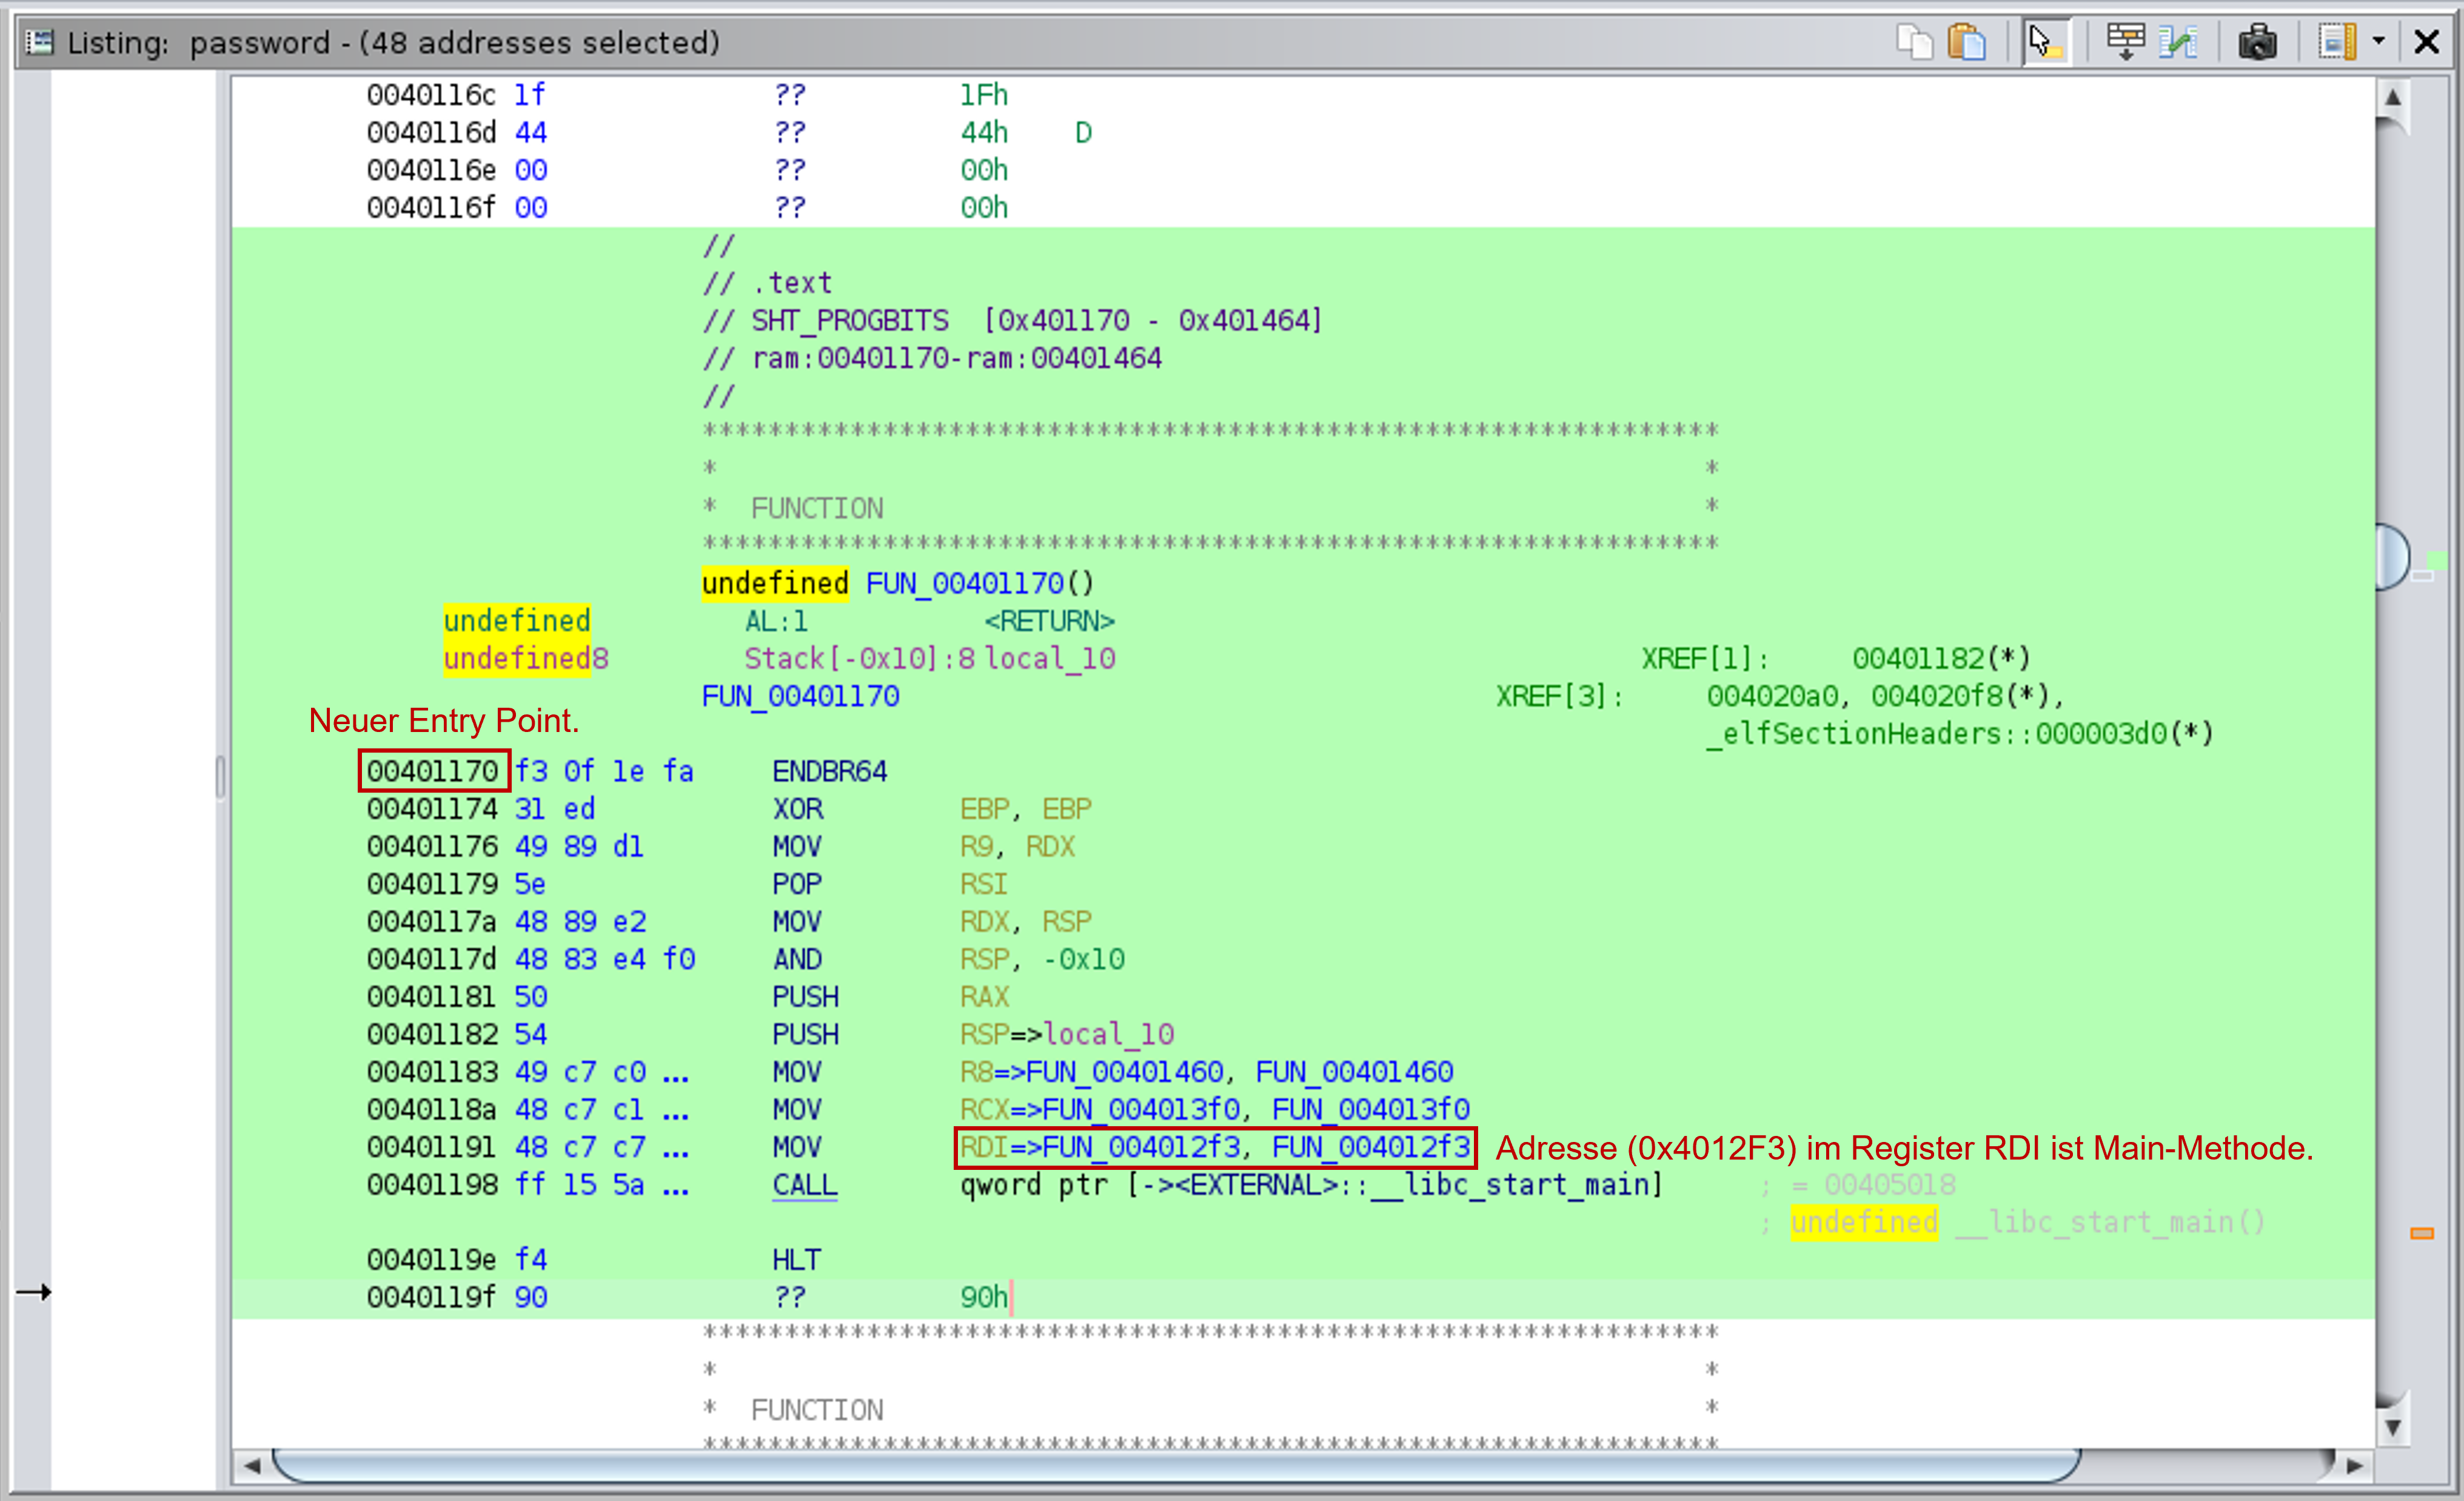
\includegraphics[width=13.5cm]{../img/Picture1.PNG}
\caption{Beginn der \textit{.text} Section.}
\end{figure}

\begin{figure} [!ht]
\centering
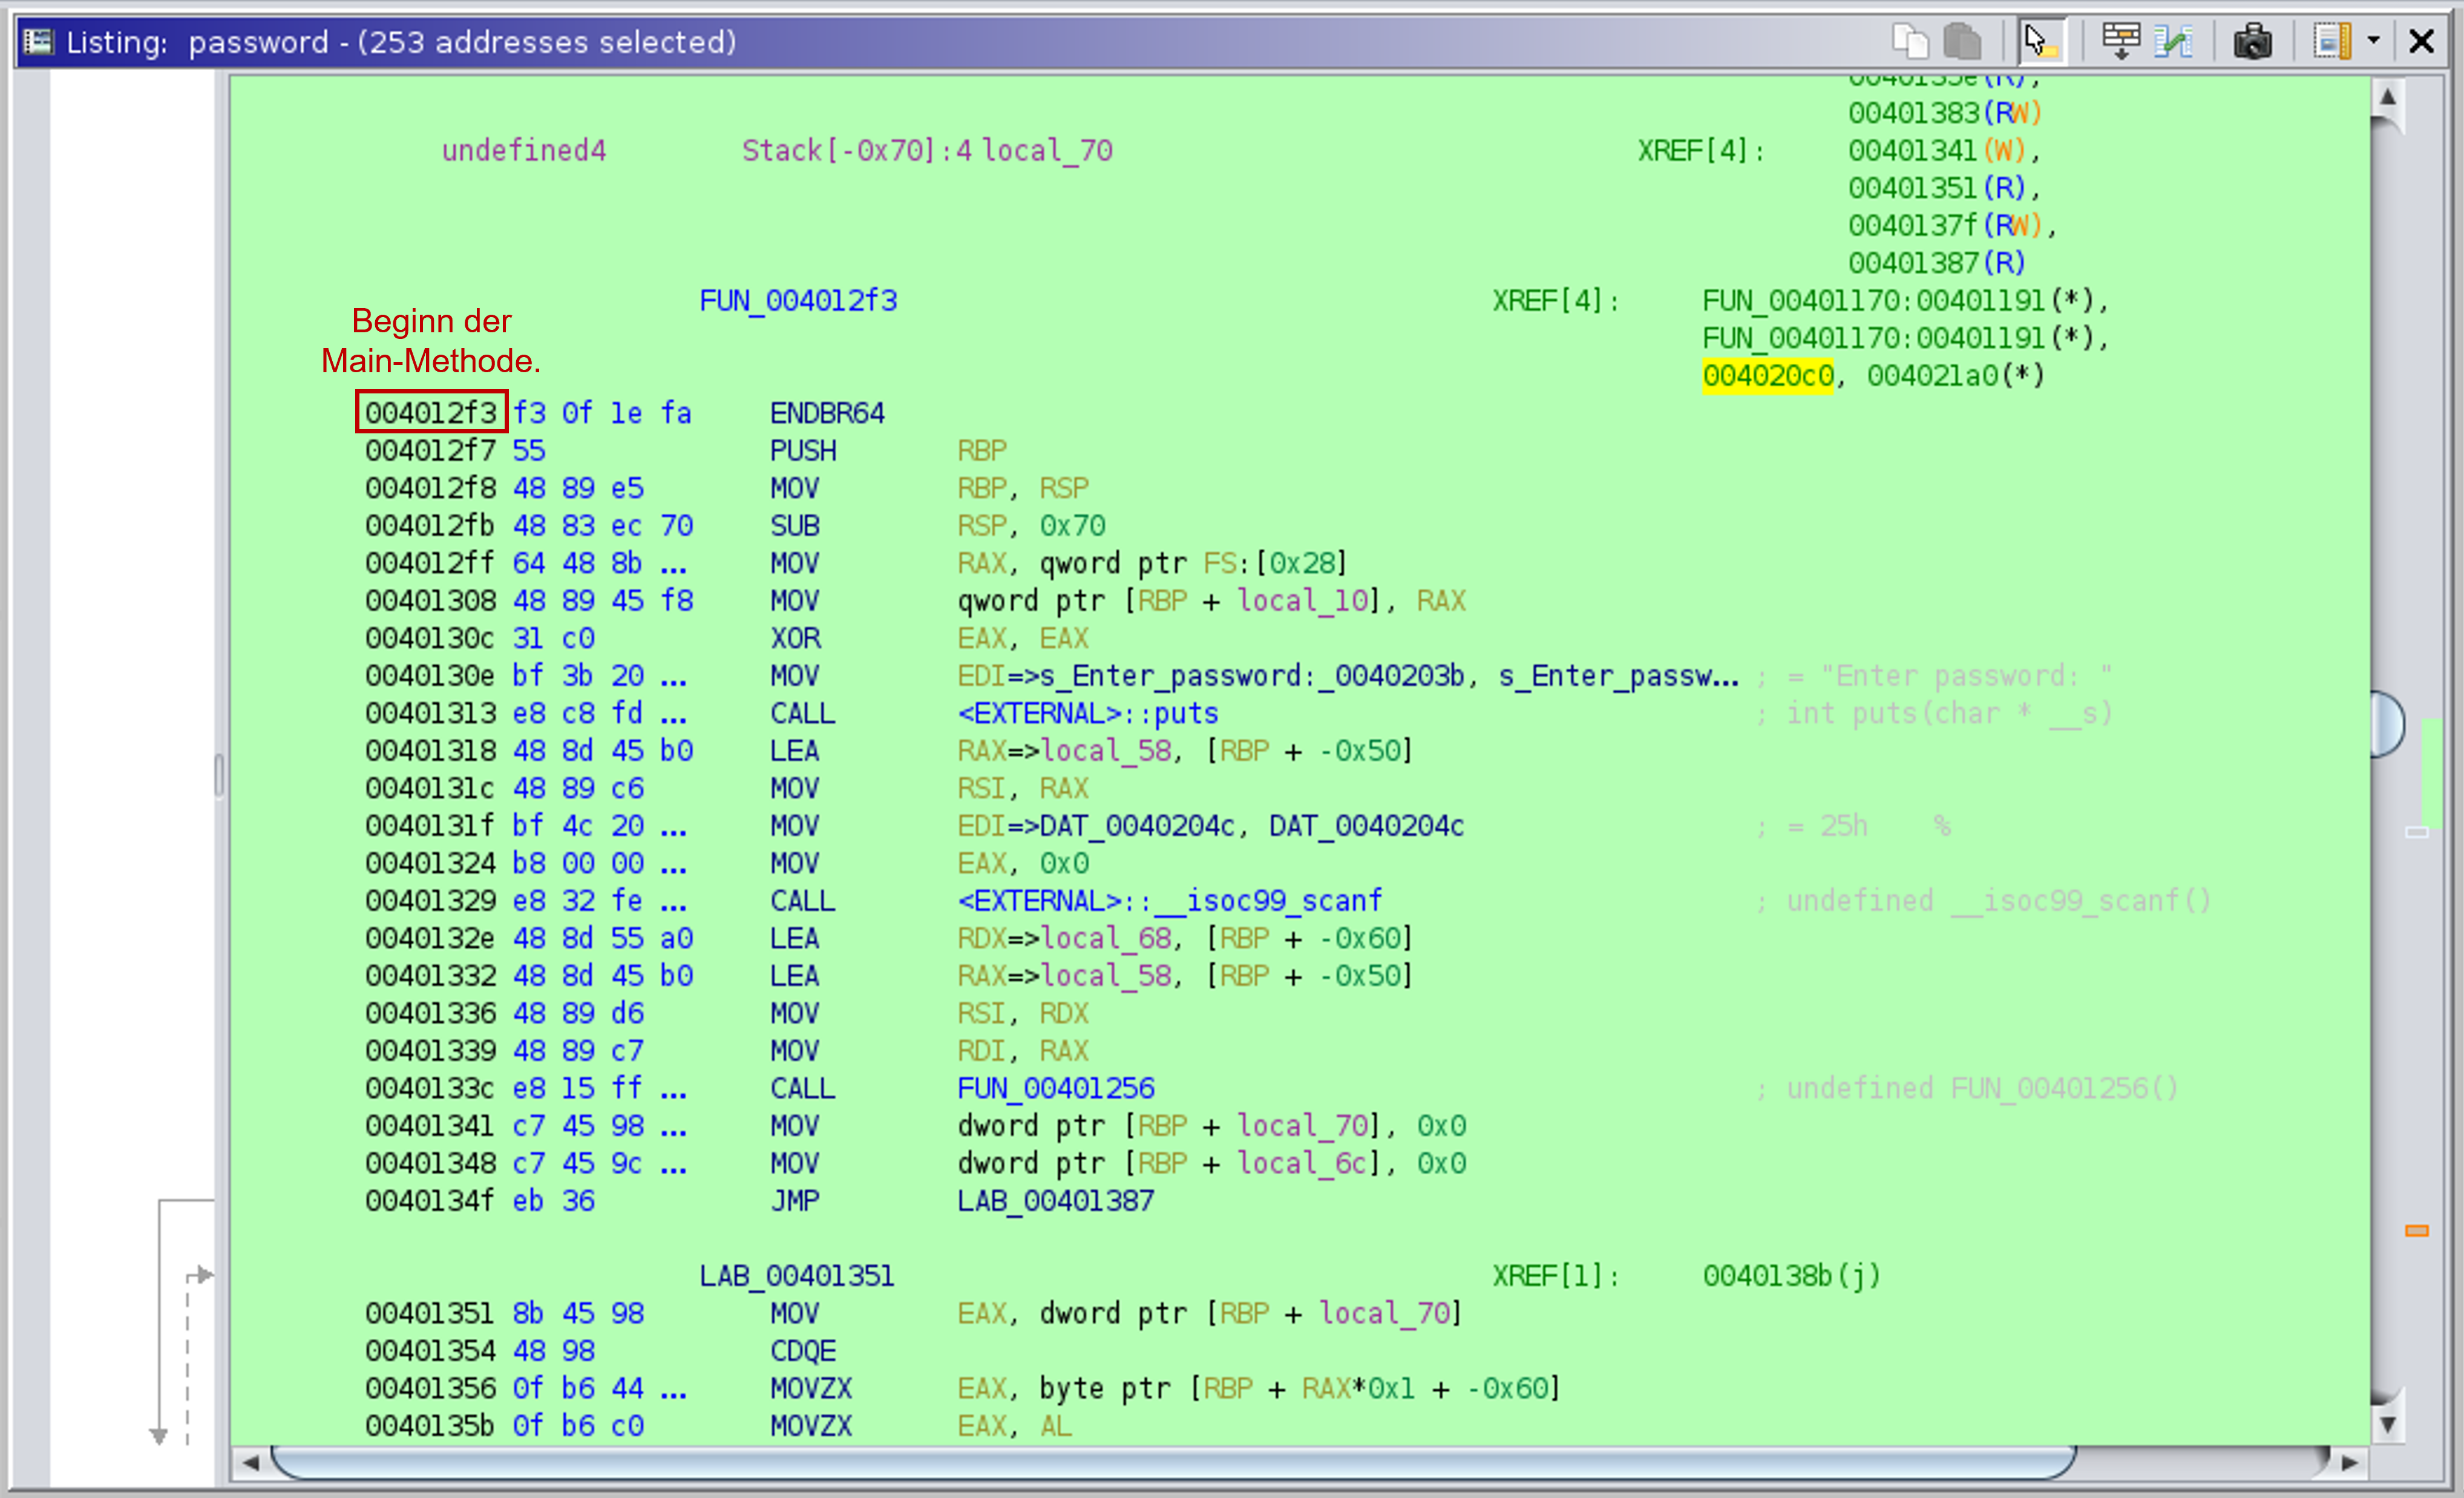
\includegraphics[width=13.5cm]{../img/Picture2.PNG}
\caption{Ausschnitt der Main-Methode.}
\end{figure}

\newpage

\subsection*{b)}

Mittels folgendem Befehl werden verlinkte Libaries angezeigt.

\begin{lstlisting}[language=bash]
    $ ldd password
\end{lstlisting}

Ausgabe:

\begin{lstlisting}
    linux-vdso.so.1
    libcrypto.so.1.1
    libc.so.6
    libdl.so.2
    libpthread.so.0
    ld-linux-x86-64.so.2
\end{lstlisting}

Wir kennen nicht die Adresse der dynamischen Symbole während der Link-Zeit, aber während der Laufzeit.
Für das dynamische Symbol wird eine Speicheradresse für die aktuelle Adresse reserviert, welche
dann während der Laufzeit gefüllt wird.

Alle dynamisch gelinkten Symbole kann man mit folgendem Befehl sehen:

\begin{lstlisting}[language=bash]
    $objdump -R password
\end{lstlisting}

Ausgabe:

\begin{lstlisting}
    DYNAMIC RELOCATION RECORDS
OFFSET           TYPE              VALUE
0000000000403ff0 R_X86_64_GLOB_DAT  __gmon_start__
0000000000403ff8 R_X86_64_GLOB_DAT  __libc_start_main@GLIBC_2.2.5
0000000000404018 R_X86_64_JUMP_SLOT  printf@GLIBC_2.2.5
0000000000404020 R_X86_64_JUMP_SLOT  puts@GLIBC_2.2.5
0000000000404028 R_X86_64_JUMP_SLOT  strlen@GLIBC_2.2.5
0000000000404030 R_X86_64_JUMP_SLOT  MD5_Final@OPENSSL_1_1_0
0000000000404038 R_X86_64_JUMP_SLOT  MD5_Update@OPENSSL_1_1_0
0000000000404040 R_X86_64_JUMP_SLOT  sprintf@GLIBC_2.2.5
0000000000404048 R_X86_64_JUMP_SLOT  __stack_chk_fail@GLIBC_2.4
0000000000404050 R_X86_64_JUMP_SLOT  strcmp@GLIBC_2.2.5
0000000000404058 R_X86_64_JUMP_SLOT  MD5_Init@OPENSSL_1_1_0
0000000000404060 R_X86_64_JUMP_SLOT  __isoc99_scanf@GLIBC_2.7
\end{lstlisting}

Beispielsweise wird bei der call Funktion am Entry Point die libc libary auf der Adresse
\textit{0x403ff8} aufgerufen.

\subsection*{c) password}

\begin{lstlisting}[language=bash]
    $ (gdb) info functions
\end{lstlisting}

Es wird die Funktion strcmp gefunden, welche Strings vergleicht. Es könnte also sein, dass
diese Funktion genutzt wird, um die Passwörter zu vergleichen.
Des Weiteren wurden noch MD5 Funktionen gefunden, welche das Passwort wahrscheinlich hashen.

Die strcmp Funktion wird gedebuggt.

\begin{lstlisting}[language=bash]
    $ (gdb) break 0x0000000000401140
\end{lstlisting}

Der Buchstabe 'e' wird eingegeben.

\begin{lstlisting}[language=bash]
    $ (gdb) info register
\end{lstlisting}

In den Registern müssten wohl das eigentliche Passwort sein und der Buchstabe 'e' in MD5 Hash.

D.h. man muss die Register einzeln als Strings ausgeben und mit einem MD5 Decrypter umkehren.
Es wird der online MD5 Decrypter von \url{https://md5decrypt.net/en/#answer} verwendet.

Es kommt raus, dass das Passwort im \textit{rdi} Register lag, welches mit folgendem Befehl ausgegeben wurde:

\begin{lstlisting}[language=bash]
    $ (gdb) x/s 0x4040a0
\end{lstlisting}

Das Password im Klartext lautet: \textit{password}

Zugehöriger MD5-Hash: \textit{5f4dcc3b5aa765d61d8327deb882cf99}

\begin{figure} [!ht]
\centering
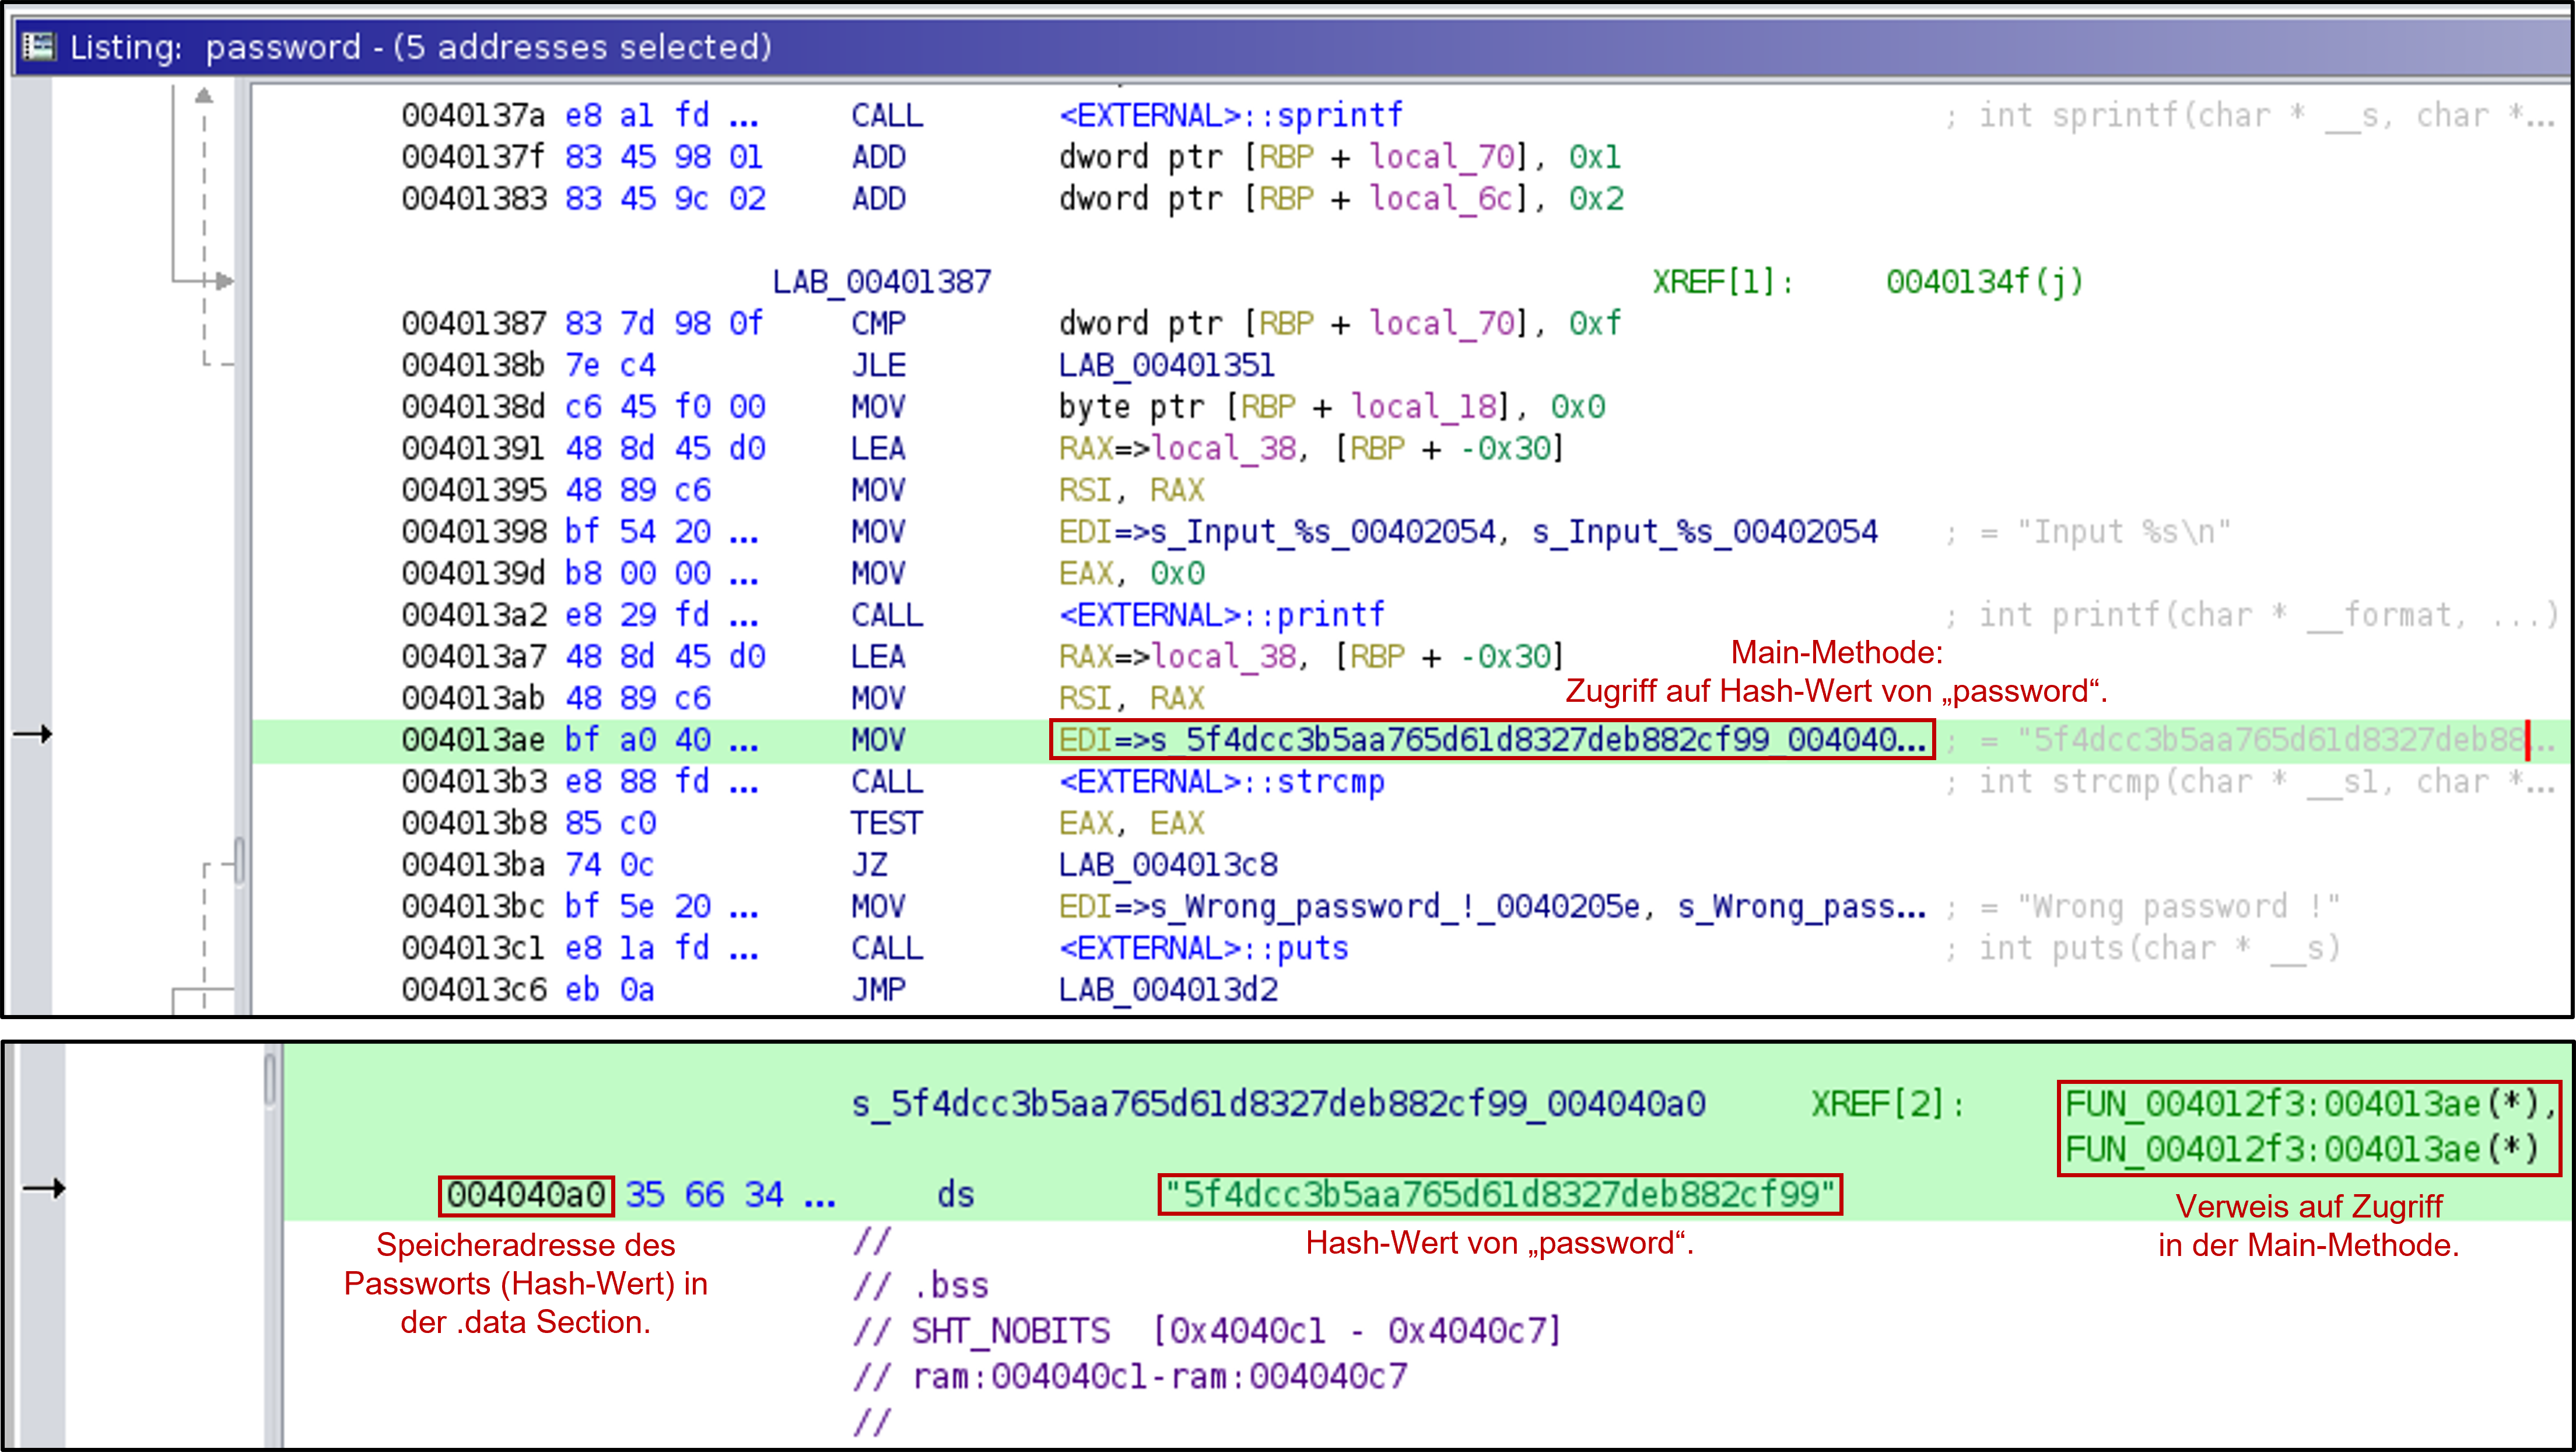
\includegraphics[width=12.5cm]{../img/Picture3.PNG}
\caption{Darstellung mittels Ghidra.}
\end{figure}

\newpage

%%%%%%%%%%%%%%
% Aufgabe 3  %
%%%%%%%%%%%%%%
\section*{Aufgabe 3 ELF Reversing}

\subsection*{a)}

\subsection*{b)}

\subsection*{c)}

\subsection*{d)}

\subsection*{e)}

\end{document}